\chapter{Installazione e accesso all'applicazione}
\label{Installazione}

\section{Requisiti di sistema}
Di seguito sono riportati i requisiti minimi di sistema che il dispositivo\glossario{Android}deve avere affinchè l'app MegAlexa venga installata: 

\begin{itemize}
	\item \textbf{Sistema Operativo}: Android 4.4 KitKat API 19;
	\item \textbf{Memoria richiesta}: 50MB;
	\item \textbf{Connessione internet}: richiesta;
\end{itemize}

\textbf{NOTA BENE:} si consiglia fortemente l'utilizzo di un dispositivo Amazon Echo per un'esperienza migliore. Se non si è in possesso di tale dispositivo c'è la possibilità di acquistarne recandosi nel sito di \href{https://www.amazon.it}{Amazon}.

\section{Installazione applicazione}
Scaricare l'app da questo \href{https://www.google.com/drive/}{link} sul proprio dispositivo
e successivamente installare il file .apk appena installato sul proprio dispositivo

\section{Avvio applicazione}
Avviare l'applicazione ed effettuare il login con il proprio account Amazon oppure creare un nuovo account Amazon seguendo la procedura guidata.
\newpage
\subsection{Iscrizione ad Amazon}

\begin{figure}[!ht]
	\centering
	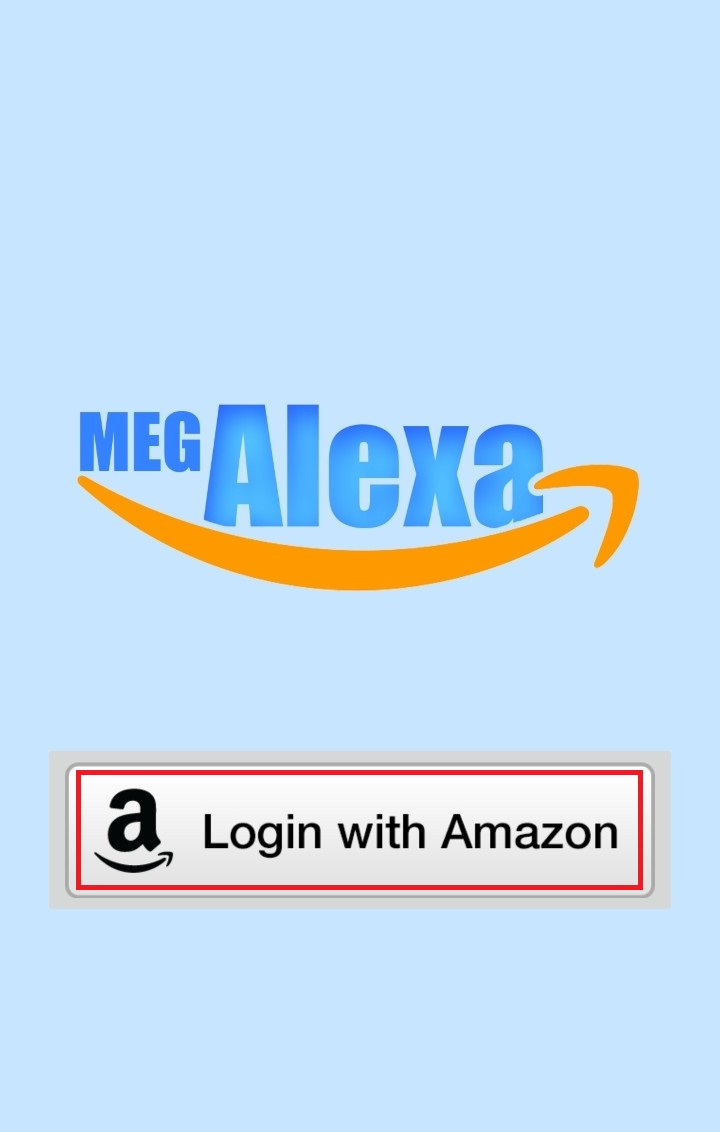
\includegraphics[scale=0.2]{images/Login.jpg}
	\caption{Pagina iniziale app}
\end{figure}
\newpage
\subsection{Login con account Amazon}

\begin{figure}[!ht]
	\centering
	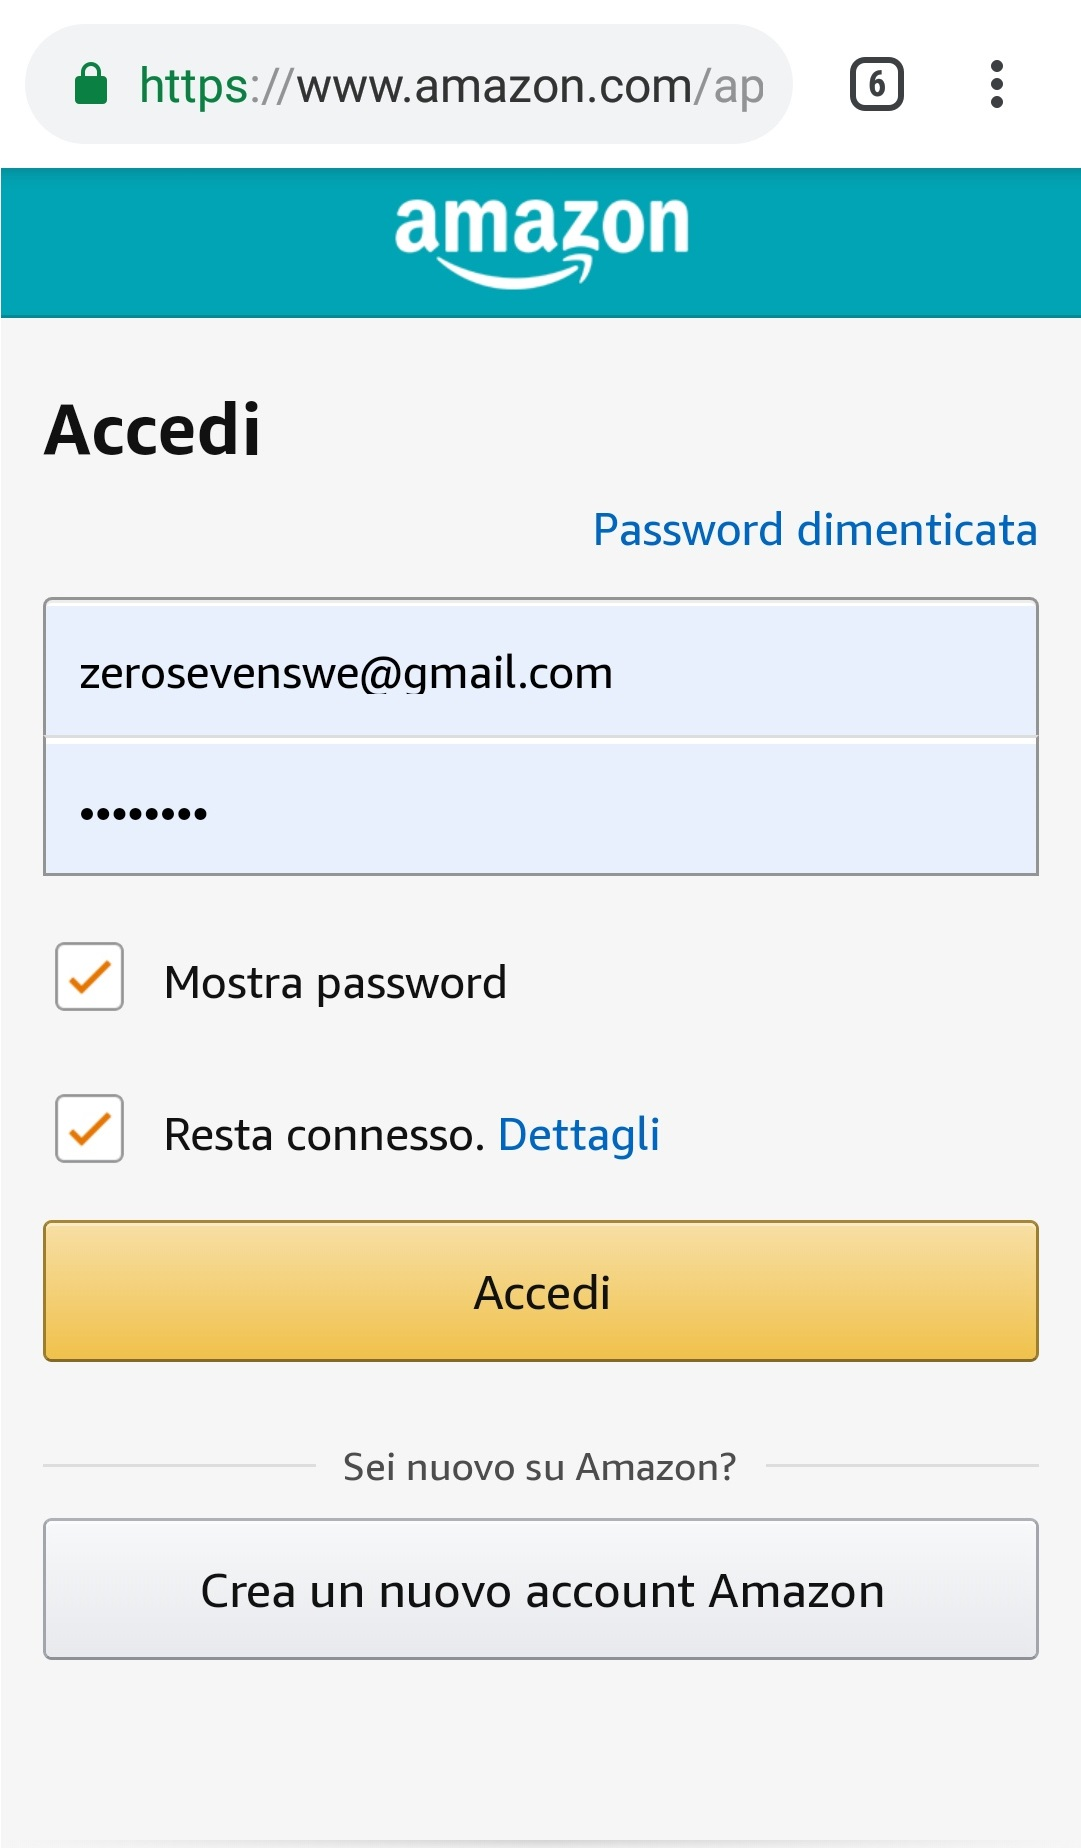
\includegraphics[scale=0.2]{images/Autentication.jpg}
	\caption{Login ad Amazon}
\end{figure}
\newpage
\subsection{Logout}

\begin{comment}
\begin{figure}[!ht]
	\centering
	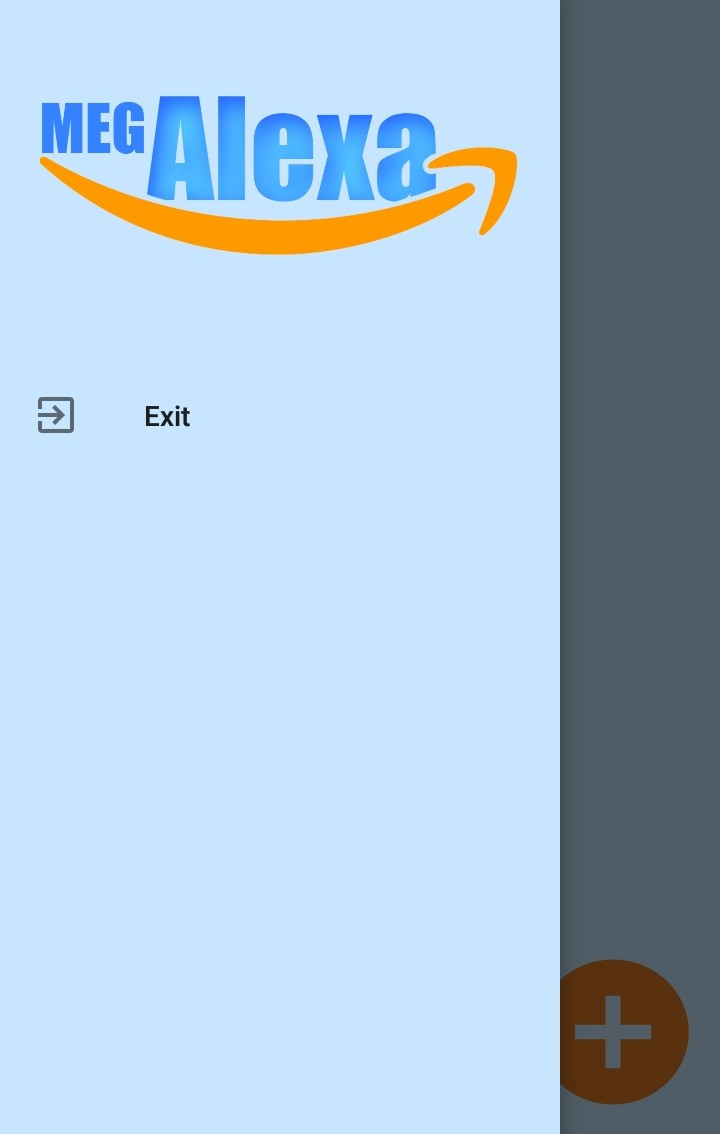
\includegraphics[scale=0.2]{images/Logout.jpg}
	\caption{Logout dall'app}
\end{figure}
\end{comment}
